\documentclass[11pt,a4paper]{article}
\usepackage[margin=1in]{geometry}
\usepackage{enumitem}
\usepackage{amsmath}
\usepackage{graphicx}
\usepackage[colorlinks=true, allcolors=blue]{hyperref}
\usepackage{fancyhdr}
\usepackage[nottoc,numbib]{tocbibind}
\usepackage{indentfirst}
\usepackage{algpseudocode}

\pagestyle{fancy}
\setlength{\headheight}{14pt}
\linespread{1.8}
\let\oldheadrule\headrule
\renewcommand{\headrule}{\color{red}\oldheadrule}
\lhead{2023 MGCS 670 Revenue Management}
\rhead{Group Assignment 1}

\title{
\large{McGill University | Desautels Faculty of Management}\\
\hfill \break
\hfill \break
\hfill \break
\hfill \break
\\\Large MGSC 670 - Revenue Management\\
\textbf{Group Assignment 1: Markdown Strategy}\\
\hfill \break
\hfill \break
}

\author{\\\\
261083570 Konstantin Volodin\\
261078897 Ying-Fang Liang\\
260658030 Emery Dittmer\\
261077392 Julie Chanzy\\\\
\hfill \break
\\\\\textbf{Instructor:} Professor Maxime Cohen\\
\hfill \break
}

\date{\emph{May 2023}}

\begin{document}

\maketitle
\thispagestyle{empty}
\pagebreak

\tableofcontents
\pagenumbering{gobble}
\pagebreak

\pagenumbering{arabic}
\setcounter{page}{1}
\section{Introduction}
Any consumer recognizes words like “discount “clearance,” or “liquidation”. Behind the scenes of these words is a carefully orchestrated price strategy, or markdown strategy. 
Economics predicts a relationship between supply, demand and price. With perfect information and competition, as the price increases the demand decreases. 
Simplified price is, therefore, a control mechanism for the quantity of an item sold. 
We will examine and predict a markdown strategy for a hypothetical retail fashion company that sells to customers (B2C). 
Within this framework, the organization holds 2,000 units of inventory with a starting price of \$60. 
The inventory must be sold within 15 weeks. There are 4 price options available, full price, -10\% -20\% and -40\% off. 
Each pricing strategy has its demand curve. This inventory-to-price scenario is illustrated in USC Marshall’s School of Business retail game \cite{RetailerGame}. 

The optimized strategy or \emph{perfect foresight strategy} maximizes the revenue generated over the 15 weeks by implementing the right markdown strategy at the right time. Since the salvage value is \$0, the maximum revenue is mathematically equivalent to a linear function of units sold at sale price. The goal is to develop a data science approach to consistently minimize the difference between the expected revenue and perfect foresight strategy.  

\section{Background}
The retail industry is playing more and more on price markdowns to optimize profit, taking into consideration the time constraint and sometimes the lack of historical data. 
Many revenue management models have tried to optimize the time and prices discounts to influence consumer behavior. 
The intuition behind is that prices drive the demand and markdowns increase reach and conversions to sales, 
Therefore, markdowns should be optimized to maximize revenue while minimizing the inventory left at the end of the sales. 
In the last decades, innovations and new data management tools have allowed companies to move away from a manual pricing system and better manage their revenues. 
\pagebreak
\begin{figure}
    \centering
    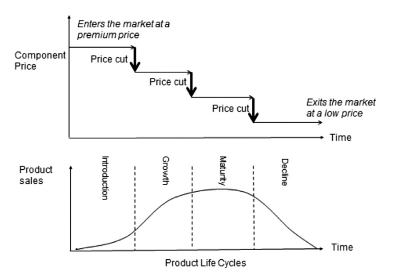
\includegraphics[width=0.75\textwidth]{pic/Picture1.png}
    \caption{Demand \& Price through Product Life Cycles.\\\cite{chung2015optimal}}
\end{figure}
\hfill \break

For example, fast-fashion retailers are looking at clearance prices strategies before liquidation \cite{caro2012clearance}, while airline carriers started managing discounted fares back in the 1970s \cite{talluri2004revenue}. 
In 2008, Zara, a multinational fast fashion company, opted to experiment with markdown strategies on multiple items. 
The model produced a 6\% or \$90M increase in sales revenue throughout the store and other cultural and business model improvements \cite{caro2012clearance}. 
The approach allows for a scalable, simple and reliable method to set pricing. 

\section{Proposed Strategies}
This case’s literature and background suggest that revenue management is more than a one-size-all approach. 
Several strategies or pricing policies may be appropriate for benchmarking and comparing different pricing methods. 
We will investigate several markdown or price change methods to understand their impact and potential application. 
We will evaluate the results using a simulation of the price and demand via a simulation based on mean price, standard deviation, and random number generation.

\subsection{Random Policy}
We will first investigate a random choice policy. 
This policy represents a likely worst-case scenario, where a company has no expertise and not logic to operate with. 
The policy will arbitrarily choose the pricing policy at each time t.  

Based on the random nature of the model and rules of the model, we expect a smaller distribution then the baseline mode (presented next). 
Since we cannot raise the price once lowered the cumulative probability of a 40\% discount approaches 50\% by the end of the 15 weeks, which is the highest of any choice. 
The distribution of revenue should largely follow the distribution of the 40\% off price distribution we have observed. 

\subsection{Baseline Model - Price Consistency}
We will investigate a naïve approach to markdown strategies: do nothing. 
We consider this a baseline model and not the most efficient one. 
More precisely, we will consider the model where we maintain the price of goods at the same level throughout the 15 weeks. 
While this naïve model may seem pointless, it is useful as a comparison point for the average revenue and standard deviation. 
In other words, the naïve “do nothing” model is a baseline to compare against and build off. 
The optimal price over the 15 weeks may be the original set price of \$60 or maybe some combination of price reductions, this model helps to determine the best approach in most situations.

We expect a highly varied revenue amount from this model that could be more consistent and optimal than the \emph{perfect foresight strategy}.

\subsection{Naïve Adaptive Likelihood Policy}
The second policy we will investigate is a naïve adaptive likelihood method that uses multiple runs of 15-week data to assume the same trends hold for future data. 
This framework generates a decision-making logic. The given data suggests that each price reduction has a compounding effect on the unit volume sold. For instance, 10\% off increases unit sales by 30\%, and 20\% increases unit sales by 75\% compared to previous periods. 
The model uses rules based on the sales increase per price category to estimate the unit sales for the remaining periods. 
If the estimated units sold by the end of the 15 weeks is less than the remaining units, the model increases the discount to stimulate the forecasted demand. 

We expect this model to have a high consistency of difference between revenue and the \emph{perfect foresight strategy}, with higher revenue than the baseline model and potential room for improvement.

\subsection{likelihood shared}

\subsection{Adaptive Likelihood Price Policy}
The third policy we will investigate is an adaptive likelihood price method. 
This method is similar to the naïve adaptive likelihood policy with a critical difference. 
Instead of using the estimated unit price increase this model aggregates the revenue from 10 separate forecasts for the remaining weeks. 
The 10 forecasts are run for each price point remaining and are based on randomly selected observed data from pervious runs.  
The model should help capture the original model’s randomness through more robust forecasts. 

We expect this model to produce a more consistent difference between revenue and the \emph{perfect foresight strategy} with a higher average revenue than the naïve adaptive likelihood policy.

\subsection{Moving Average Naïve}
Next, we will investigate a naive moving average approach. 
In this approach the previous 3-day demand is accumulated into a moving average to forecast demand.
The 3-day average helps smooth any randomness in the demand curve due to noise. 
The function considers the remaining time and the momentum of previous sales to determine if the current trajectory of sales will result in no inventory at the end of the 15 week period. 
If the sales momentum from the previous 3 days is lower than the average number of units needed to sell out by the end of the period, the price is dropped. 
Let’s consider an example: at week 4, the previous 3 weeks sales average is 100 units per week. There are 1700 units left. 
The average sales needed to sell out of inventory is 141 units (1,700units/ 12 weeks). 
Since the moving average sales (100 per week) is below the required 141 sales per week the model will lower the price. 
The following week the model will re-examine the same factors to decide whether to lower the price once again or not. 
This simple model accounts for the randomness of demand and helps to ensure more unit sales by valuing unit sales momentum over optimal price strategy.

We expect this model to have a higher consistency than the baseline mode, lower the price quickly to the lowest amount and consistently sell out of all units. This model is likely better than the baseline but could be better.

\subsection{Adaptive Moving Average with Wait}
The final policy we will investigate is an adaptive moving average with a waiting policy. 
This policy is similar to the naïve moving average policy with added levels of complexity. 
The moving policy is at risk of quickly devolving to the lowest price policy as previous price changes may not have time to take effect. 
Therefore, the model will wait until 3 weeks after the previous price change, to allow for the previous price changes to take effect.

We expect this model to have a lower difference consistency than the naïve average, since it is likely that more of the units sold will be at different price points whereas the average model will have over 50\% of the units sold for the maximum or minimum price. 
However, we also expect that this model will result in the highest average revenue from all models.

\subsection{Reinforcement Learning}
Some artificial intelligence models rely on supervised reinforcement learning which learn as they go. 
The models are rewarded for certain actions and attempt to maximize the reward, relying on previous runs or iterations to build off of. 
These models are ideal for repeated tasks that have defined conditions. 
For example, Open Ai in 2019 demonstrated a reinforcement learning model that simulated a game of hide and seek \cite{baker2019emergent}.
We will apply reinforcement learning to this problem, where the reward function is the maximization of the revenue, and the inputs are the app itself. 
While this model offers little explanation ability since rl models are black box models, the reinforcement learning policy may perform better than previous policies. 

We expect that the reinforcement learning model will have the highest revenue and the lowest revenue distribution of all models previously tested. 

\section{Implementation}

\subsection{Data Treatment}
While we have access to 15 runs of “historical” data, before using this data, we must apply data preprocessing. 

First, we must ensure that the data does not contain errors or null values. 
We, therefore, removed null rows and appended the run number (1-15) to each observation within the data. 
After the data cleanup, we are left with a dataset containing the run number, the week number, the price of the item (\$60, \$54, \$48, \$36), the unit demand and the revenue generated from that week of sales. 

Second, we need to transform the data into more meaningful formats. 
We grouped the data by price to measure unit sales’ standard deviation and mean. 
This first grouping was helpful in the naïve price policy we applied. 
We also grouped the data by price to measure the mean and standard deviation of the unit sales compared to the previous week. 
In other words, what is the \% increase (or decrease) in unit sales when a new price point is set. It may be that a 20\% decrease in price increases unit sales by 70\%, independent of the previous price point. 

Based on some casual observations of the data, the distributions appear roughly normally distributed, we will use this as a basis for simulation and modelling. 

\subsection{Simulation}
To forecast the impact of the pricing strategies we are investigating, we must test the policies against data. 
Since we cannot access the exact equation or similar random number generator used for the web app, we must first utilize simulations. 
The model built takes the policy, the average and the standard deviation of the observed price points and generates 100 simulations. 
For each simulation and each time t, the model generates unit sales based on a numpy random normal method using the mean and standard deviation of the current price point. 
The simulation approach best reflects a real-life scenario as a forecast function is generally unknown, resulting in a reliance on past data to predict future demand. 
The generated numbers reflect the data distribution found within the historical data. \\

\begin{itemize}[leftmargin=*]
    \item Pseudo Code of Simulation Approach and Validation
\end{itemize}

\begin{algorithmic}[1]
    \Procedure{Simulate}{$means\ per\ price,\ stdev\ per\ price$}
        \For{week in length($means\ per\ price$)}
            \State \textbf{generate} unit sales \textbf{with} mean, stdev
        \EndFor
        \State \textbf{return} unit sales
    \EndProcedure
    \State 
    \Procedure{Test Policy}{$policy,\ list\ of\ unit\ sales$}
        \For{t = 1 to 15}
            \State \textbf{generate} price at week t+1 from $policy$ logic
        \EndFor
        \State \textbf{return} price at week t+1
    \EndProcedure
    \State
    \For{policy in policy candidate list}
        \For{t = 1 to 100}
            \State list of unit sales = $Simulate$ (price mean, price stdev) 
            \State policy results = $Test\ Policy$ (policy, list of unit sales) 
        \EndFor
    \EndFor
\end{algorithmic}

\subsection{Validation}
The simulation approach helps validate the models and quickly select the best policy with limited information. 
However, for this context, we need not rely solely on the simulation data, we can instead use the actual data from the web app. 
The assumptions and approach we have previously laid out may have unknown challenges or other pitfalls. 
In this scenario we are not limited to the simulation and approximation of “real world data”. 
We will therefore validate the simulation results using the web application. 
To implement the validation, we will utilize a selenium-based python script which goes between the code and user interface on the web app. 
Each policy is tested in real-time against the app while recording the results to evaluate after the fact. \\

\begin{itemize}[leftmargin=*]
    \item Pseudo Code of Policy Validation using WebApp
\end{itemize}

\begin{algorithmic}[1]
    \Procedure{Policy Validate}{$policy$}
        \State URL = "http://www.randhawa.us/games/retailer/nyu.html"
        \State expected return = \textbf{with} URL \textbf{use} $policy$ for t+1 decision
        \State \textbf{return} expected return
    \EndProcedure
    \State
    \For{policy in policy candidate list}
        \For{t = 1 to 100}
            \State policy results = $Policy\ Validate$ (policy) 
        \EndFor
    \EndFor
    \State \textbf{plot} policy results
\end{algorithmic}
\pagebreak

\section{Discussion and Recommendations}

\subsection{Policy Comparison}

\subsection{Recommended Policy}

\pagebreak
\bibliographystyle{apalike}
\bibliography{ref.bib}

\end{document}